
\chapter{Experiments and Results}\label{ch:results}

\section{Introduction}\label{sec:res:intro}

A vision-language-action policy that is competent at manipulation is not thereby safe, and the
standard remedy --- a control barrier function shield correcting its actions at every step ---
remains attached for the life of the deployment. This study asks whether those corrections can
instead be compiled into the policy, so that the shield is no longer required
(Section~\ref{sec:intro:rationale}).

The method is the controlled comparison set out in Chapter~\ref{ch:method}: a shield is built over
$\pi_{0.5}$, its corrections are collected as demonstrations, those demonstrations are
behaviour-cloned back into the policy's action head, and the result is evaluated with the shield
removed. Every condition reported here is $n = 120$ rollouts on held-out initial states, with
proportions given as Wilson 95\% intervals and differences read from interval overlap
(Section~\ref{sec:method:analysis}).

This chapter presents what those experiments produced. It reports the measurements and states what
each contributes to the research questions of Section~\ref{sec:intro:rationale}; the interpretation
of what they mean, and how they sit against the literature, is deferred to
Chapter~\ref{ch:discussion}.

The chapter follows the research questions in order. Section~\ref{sec:shield_efficacy} establishes
whether the shield works at all (RQ1) and Section~\ref{sec:res:internalise} whether its effect
survives distillation (RQ2). Sections~\ref{sec:res:mechanism} and~\ref{sec:res:source} address what
determines whether the transfer occurs, first by isolating the shield from outcome selection and
then by varying the demonstration source (RQ3). Sections~\ref{sec:res:scope}
and~\ref{sec:res:channels} report what the transfer does not cover and whether alternative
mechanisms succeed where it does not (RQ4).

\section{The Demonstration Sets}\label{sec:res:demos}

Three demonstration sets were collected, and every distillation result reported in this chapter
draws on one of them. Their composition is given in Table~\ref{tab:demo_sets}.

\begin{table}[htbp]
\centering
\begin{threeparttable}
\caption[Composition of the demonstration sets]{%
  The three demonstration sets. Yield is the fraction of collection rollouts passing the retention
  filter. Activation rate and correction norm characterise how much the shield altered the
  trajectories that were kept.}
\label{tab:demo_sets}
\begin{tabular}{lrrrrcc}
\toprule
\textbf{Set} & \textbf{Demos} & \textbf{Rollouts} & \textbf{Yield} & \textbf{Scenes}
  & \textbf{Activation} & \textbf{Corr.\ norm} \\
\midrule
Shielded self-rollouts\tnote{a}  & 186 & 480 & 39\% & 24 & 0.32 & 0.33 \\
Privileged planner\tnote{b}      & 318 & 864 & 37\% & 18 & ---  & ---  \\
Unshielded control\tnote{c}      & \phantom{0}85 & 480 & 18\% & 24 & 0    & ---  \\
\bottomrule
\end{tabular}
\begin{tablenotes}[flushleft]\footnotesize
\item[a] Retained if the episode succeeded, displaced nothing, and the shield intervened at least
  once. Activation is the median fraction of control steps shielded; the median episode carries 51
  interventions, the minimum nine, and none fewer than five. Correction norm is measured against
  actions bounded to $\pm 1$ per axis.
\item[b] Retained if the episode succeeded and displaced nothing. Six of the 24 scenes produced no
  usable demonstrations (Section~\ref{sec:res:source}).
\item[c] Collected with the shield switched off and filtered on the same success and displacement
  criteria; the shield-intervened criterion is inapplicable. Used in
  Section~\ref{sec:res:mechanism}, where the shielded set is subsampled to 85 to match.
\end{tablenotes}
\end{threeparttable}
\end{table}

Two features of the table bear on results reported later. The shielded set is pervasively
corrected: the barrier is active on roughly a third of control steps in the median episode, moving
the action by 0.33 against a bound of $\pm 1$. And collecting safe demonstrations without the
shield is roughly twice as expensive, at an 18\% yield against 39\%.



\section{Does the Shield Make \texorpdfstring{$\pi_{0.5}$}{pi 0.5} Safe?}\label{sec:shield_efficacy}

The first question is whether a control barrier function shield, applied as a runtime filter, makes
a pretrained VLA safe on this benchmark at all. Table~\ref{tab:shield_efficacy} reports the
comparison: the shield removes 69 percentage points of collision, with disjoint confidence
intervals.

\begin{table}[htbp]
\centering
\caption{Safety and task performance for base $\pi_{0.5}$ with and without the CBF runtime shield.
  Pooled over 24 scenes, $n = 120$ held-out rollouts per condition, Wilson 95\% intervals.}
\label{tab:shield_efficacy}
\begin{tabular}{lccc}
\toprule
\textbf{Policy} & \textbf{TSR (95\% CI)} & \textbf{Collision rate (95\% CI)} & \textbf{CAR} \\
\midrule
Base, no shield & 58.3\% [49.4, 66.8] & 82.5\% [74.7, 88.3] & 17.5\% \\
Base + shield   & 71.7\% [63.0, 79.0] & 13.3\% [\phantom{0}8.4, 20.6] & 86.7\% \\
\bottomrule
\end{tabular}
\end{table}

Success also rises, from 58.3\% to 71.7\%. That direction is worth noting, because in
Section~\ref{sec:res:internalise} the same shield applied to an already-avoidant policy lowers
success instead.

\paragraph{Answering RQ1.}
A control barrier function shield does make a pretrained vision-language-action policy safe on this
benchmark: collisions fall by 69 percentage points with disjoint intervals, and task success rises
rather than degrades. The corrections it applies are therefore large enough to constitute a
training signal, which is the precondition for everything that follows.

\section{Can the Shield's Safety Be Internalised?}\label{sec:res:internalise}

The shielded demonstration set of Table~\ref{tab:demo_sets} was behaviour-cloned into the policy's
action head, and the procedure was repeated for a second round.

\begin{figure}[htbp]
  \centering
  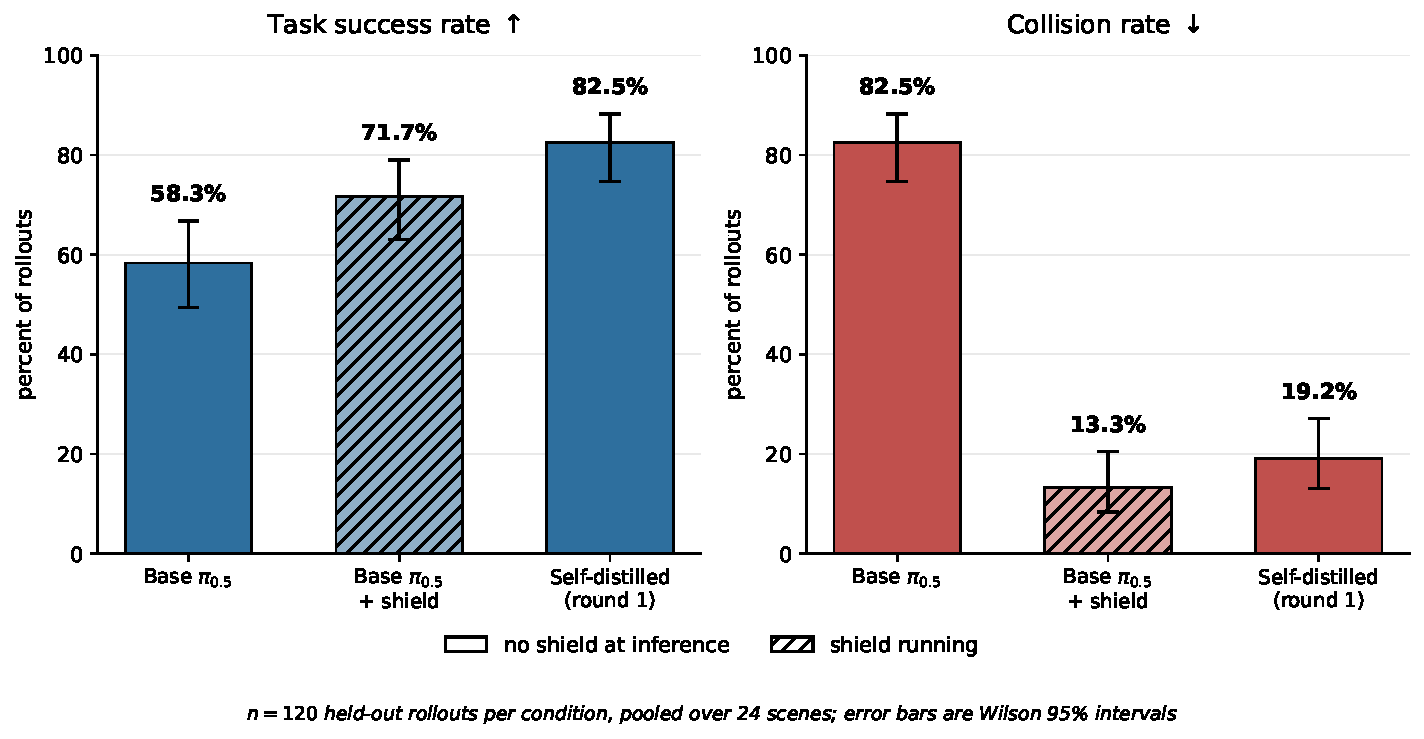
\includegraphics[width=\linewidth]{figures/fig_internalisation.pdf}
  \caption[Internalisation of the shield's safety]{%
    The central result. The self-distilled policy, running with \emph{no shield at inference}
    (solid), is both safer and more successful than the base policy it was distilled from, and
    recovers most of the safety of the shielded baseline (hatched). Error bars are Wilson 95\%
    intervals at $n = 120$ held-out rollouts per condition.}
  \label{fig:internalisation}
\end{figure}

\begin{table}[htbp]
\centering
\begin{threeparttable}
\caption[Effect of self-distillation on safety and task performance]{%
  Effect of self-distillation, with and without the shield at inference. Rows in bold are the
  shield-free distilled policies, which are the claim of this work. $n = 120$ held-out rollouts
  per row, pooled over 24 scenes; intervals are Wilson 95\%.}
\label{tab:internalisation}
\begin{tabular}{lcccrr}
\toprule
\textbf{Policy} & \textbf{TSR (95\% CI)} & \textbf{Collision (95\% CI)} & \textbf{CAR}
  & \textbf{CBF act.}\tnote{a} & \textbf{ETS}\tnote{b} \\
\midrule
Base, no shield        & 58.3\% [49.4, 66.8] & 82.5\% [74.7, 88.3] & 17.5\% & ---   & 138.6 \\
Base + shield          & 71.7\% [63.0, 79.0] & 13.3\% [\phantom{0}8.4, 20.6] & 86.7\% & 0.355 & 160.6 \\
\addlinespace[3pt]
\textbf{Round 1, no shield} & \textbf{82.5\% [74.7, 88.3]} & \textbf{19.2\% [13.1, 27.1]}
  & \textbf{80.8\%} & --- & 157.3 \\
Round 1 + shield       & 70.8\% [62.2, 78.2] & \phantom{0}8.3\% [\phantom{0}4.6, 14.7] & 91.7\% & 0.177 & 170.0 \\
\addlinespace[3pt]
\textbf{Round 2, no shield} & \textbf{80.8\% [72.9, 86.9]} & \textbf{17.5\% [11.7, 25.3]}
  & \textbf{82.5\%} & --- & 158.8 \\
Round 2 + shield       & 72.5\% [63.9, 79.7] & \phantom{0}9.2\% [\phantom{0}5.2, 15.7] & 90.8\% & 0.182 & 176.7 \\
\bottomrule
\end{tabular}
\begin{tablenotes}[flushleft]\footnotesize
\item[a] CBF activation rate (Section~\ref{sec:metrics}): the fraction of control steps on which
  the shield altered the action. Inapplicable when no shield is running, shown as ---.
\item[b] Execution time to success, in control steps, over successful rollouts only
  (Section~\ref{sec:metrics}). Conditional on success and must be read alongside TSR.
\end{tablenotes}
\end{threeparttable}
\end{table}

The headline result is the third row. With no shield running at inference, the distilled policy
displaces the obstacle in 19.2\% of episodes, against 82.5\% for the policy it was distilled
from~--- and its success rate rises from 58.3\% to 82.5\%. Both intervals are disjoint from the
base policy's. The distilled policy is simultaneously safer and more capable than its own teacher,
without the teacher's filter.

It is worth noting how close this comes to the shielded baseline: CAR 80.8\% shield-free against
86.7\% with the shield active. Most of the shield's safety benefit survives its removal.

\paragraph{One round is enough.}
Rounds one and two overlap on both metrics, so the second round buys nothing measurable. It also
does not erode performance.

\paragraph{Stacking the shield costs success.}
Applying the shield to the distilled policy lowers collisions further, to 8.3\%, but reduces success
from 82.5\% to 70.8\%. This is the reverse of the effect in Section~\ref{sec:shield_efficacy}, where
the same shield raised success. The two observations are reconciled in
Section~\ref{sec:disc:cost}.

\paragraph{The cost of internalised caution.}
ETS rises from 138.6 to 157.3 steps, roughly 14\% slower. The distilled policy takes a more
conservative route.

\paragraph{Answering RQ2.}
The shield's safety is internalised. With no shield at inference the distilled policy collides in
19.2\% of episodes against the base policy's 82.5\%, and succeeds in 82.5\% against 58.3\%, both
intervals disjoint. It recovers most of the shielded baseline's collision avoidance (80.8\% against
86.7\%) without the filter, in a single round, at a cost of roughly 14\% in execution time.

\begin{figure}[htbp]
  \centering
  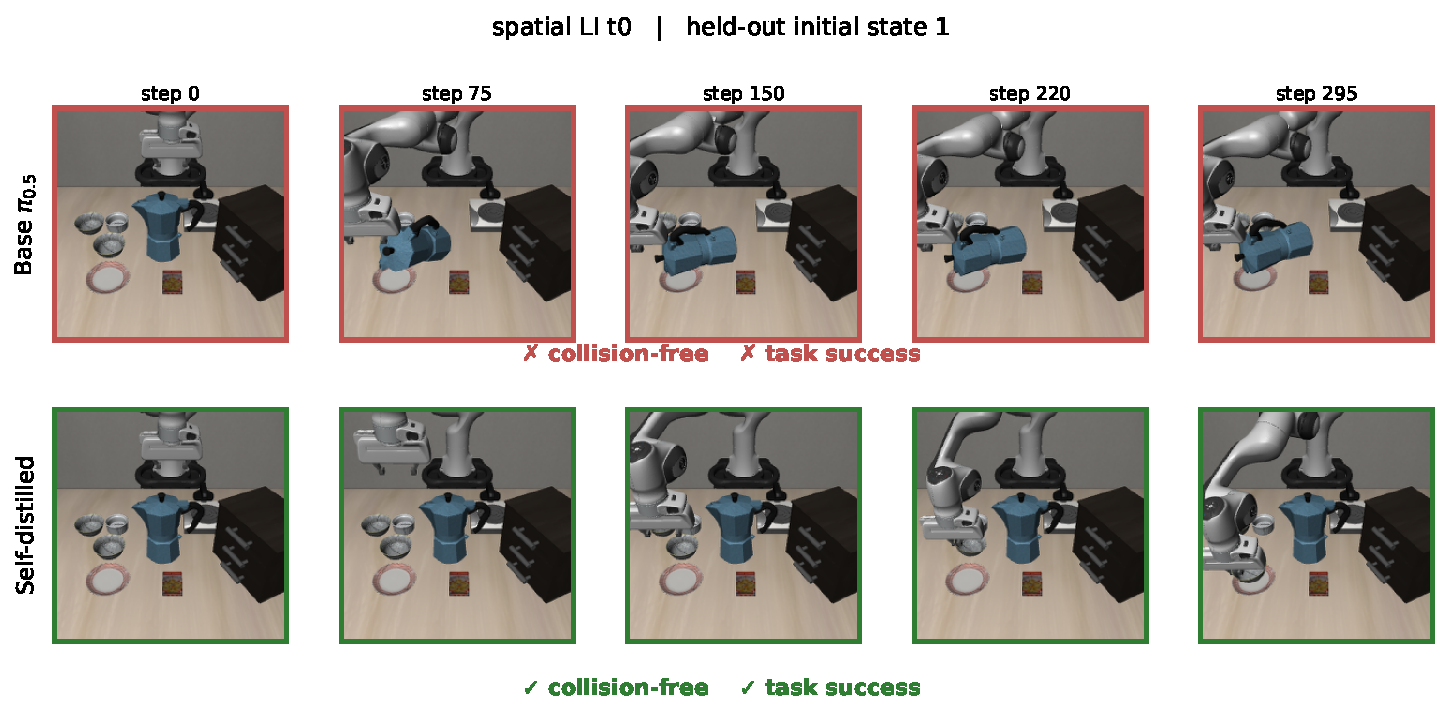
\includegraphics[width=\linewidth]{figures/fig_filmstrip.pdf}
  \caption[The same scene under the base and distilled policies]{%
    The same scene and the same held-out initial state under the base policy (top) and the
    self-distilled policy (bottom), neither running a shield. Frames are sampled at equal fractions
    of each episode: the base rollout runs to the horizon without completing, while the distilled
    rollout finishes at step 168.}
  \label{fig:filmstrip}
\end{figure}

\section{What Explains the Improvement?}\label{sec:res:mechanism}

Section~\ref{sec:res:internalise} showed that distilling the shielded policy's own clean rollouts
makes it dramatically safer without the shield; however, it does not explain why this is so. The
demonstrations were filtered on three properties at once --- the shield fired, the episode
succeeded, and nothing was displaced --- and two mechanisms are conflated in the filter.

Under the first, \textbf{distillation}, the policy imitates the shield's avoidance corrections.
This is the claim of this work. Under the second, \textbf{selection}, the improvement comes from
training a policy on its own successful episodes, a known self-improvement effect requiring no
shield. If the second mechanism accounts for the result, the shield is incidental and the contribution is a
rediscovery of filtered behaviour cloning.

To disambiguate this, a matched control was run.

\subsection*{The matched control}

The matched control held every variable constant except for switching off the shield when collecting the demonstrations.


\begin{table}[htbp]
\centering
\caption{The matched control. Both distilled conditions use 85 demonstrations passing an identical
  filter; they differ only in whether the shield was active during collection. $n = 120$ held-out
  rollouts per row, Wilson 95\% intervals.}
\label{tab:matched_control}
\begin{tabular}{lccc}
\toprule
\textbf{Condition} & \textbf{Demos} & \textbf{TSR (95\% CI)} & \textbf{Collision (95\% CI)} \\
\midrule
Undistilled base & ---            & 58.3\% [49.4, 66.8] & 82.5\% [74.7, 88.3] \\
Control, shield \textbf{off}  & 85 & 50.0\% [41.2, 58.8] & 84.2\% [76.6, 89.6] \\
Matched, shield \textbf{on}   & 85 & \textbf{75.8\% [67.4, 82.6]} & \textbf{26.7\% [19.6, 35.2]} \\
\bottomrule
\end{tabular}
\end{table}

Compared to the base policy, the control has a marginally worse collision rate and more substantial TSR degradation. So, success-filtering by itself is unsuccessful in this benchmark. At the same demonstration count and under the same filter, the shielded condition reaches 26.7\%, with a confidence interval disjoint from the control's. Therefore, the difference between the two conditions is attributable to the shield. The activation rate corroborates this independently: after distillation the shield finds materially less to correct (Table~\ref{tab:internalisation}), and a policy that merely succeeded more often would not require \emph{less} safety intervention.

The control is not uniformly inert, however. Per-body attribution shows its arm-link collisions
falling from 17 to 6 while gripper collisions remain at 44, which is why the total did not move.
Outcome selection therefore transfers avoidance in the channel the barrier does not express, while
leaving the channel that dominates the collision count unchanged.

\paragraph{Answering RQ3, first part.}
The improvement is produced by the shield's corrections, not by training on successful episodes.
At matched demonstration count and under an identical filter, collection with the shield switched
off leaves the policy indistinguishable from the undistilled baseline, while collection with it
active produces a disjoint improvement.

\section{Does the Source of the Demonstrations Matter?}\label{sec:res:source}

Section~\ref{sec:res:mechanism} established that the shield's corrections, rather than outcome
selection, produce the transfer. This section asks whether it matters whose rollouts those
corrections are applied to. A sampling-based motion planner was used as an alternative teacher:
RRT-Connect in joint space with clearance inflation, followed by inverse kinematics and playback as
operational-space deltas (Section~\ref{sec:teacher_planner}).

\begin{table}[htbp]
\centering
\caption{Comparison of demonstration sources for policy distillation.}
\label{tab:demo_source_comparison}
\begin{tabular}{lcc}
\toprule
\textbf{Policy} & \textbf{TSR (95\% CI)} & \textbf{Collision rate (95\% CI)} \\
\midrule
Base, no shield                     & 58.3\% [49.4, 66.8] & 82.5\% [74.7, 88.3] \\
Planner-distilled, no shield        & 54.2\% [45.3, 62.8] & 80.0\% [72.0, 86.2] \\
Self-distilled (round 1), no shield & \textbf{82.5\% [74.7, 88.3]} & \textbf{19.2\% [13.1, 27.1]} \\
\bottomrule
\end{tabular}
\end{table}

The planner-distilled policy is statistically indistinguishable from the undistilled base policy on
both metrics and the only variable is the demonstration source (Section~\ref{sec:distillation}).

An interactive DAgger variant was also attempted and is reported in Appendix~\ref{app:dagger}; it did not alter the conclusion of the matched comparison below.

\paragraph{The planner is not a weaker teacher.}
It might be supposed that the planner's demonstrations simply contain less safety information.
They do not. Run unshielded on spatial task~0 the expert collides in 5 of 8 episodes, with
contact from arm links, gripper, held object and scene objects alike; run shielded it collides
in none. Its demonstrations depend on the shield to the same degree the policy's own do, and
both sets were collected under it. The demonstration sets are therefore matched in correction
signal, and differ in the states they occupy.


\paragraph{The mechanism is state coverage.}
Figure~\ref{fig:state_coverage} takes the base policy's own visited states and asks
how closely each demonstration set approaches them.

Subsampled to equal size per scene, the shielded rollouts cover 37.7\% of the policy's own
states within 2\,cm against the planner's 22.8\%, and cover better in 15 of the 18 scenes
holding both demonstration types. Without that control the two sets are near-indistinguishable
at 37.7\% against 32.8\%, so the matching is load-bearing rather than cosmetic.

Figure~\ref{fig:state_coverage}(b) shows the shape of the difference. The planner is a
scripted controller and traces near-identical paths from a given initial condition, so its
demonstrations form tight deterministic bands; the states the policy actually visits are diffuse
and lie largely between and around them. The two distributions are not disjoint, but the planner's density is concentrated where the policy is not.

Two limits apply. Coverage is measured on end-effector position, 3 of the 8 observed dimensions,
so it says nothing about joint configuration. And it is descriptive rather than causal: the
matched comparison establishes that the demonstration source mattered, while the coverage figure
proposes how the two sources differ.

\begin{figure}[htbp]
  \centering
  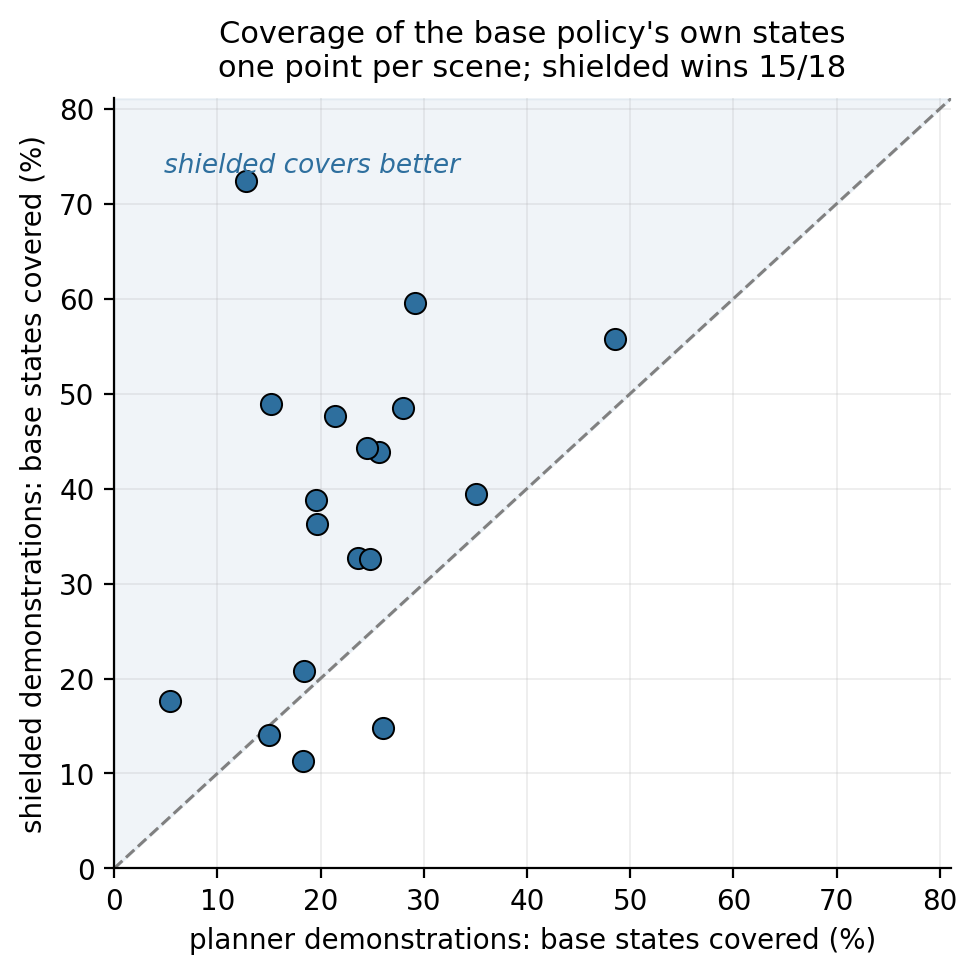
\includegraphics[width=\linewidth]{figures/fig_state_coverage.png}
  \caption[State coverage of the base policy's own trajectories]{%
    Both
    demonstration sets are subsampled to equal size per scene (30 resamples).
    \textbf{(a)} The shielded rollouts cover the policy's own states
    better in 15 of 18 scenes, 37.7\% against 22.8\% pooled.
    \textbf{(b)} The same comparison on the widest-gap scene. The planner's demonstrations
    form tight, near-deterministic trajectory bands, while the states the policy actually
    visits are diffuse and largely elsewhere.}
  \label{fig:state_coverage}
\end{figure}

\paragraph{Observation aliasing, tested and rejected.}
The intuitive explanation for that failure is that the shield's corrections
depend on state the policy cannot see: $\pi_{0.5}$ observes an image and eight proprioceptive
dimensions but no joint angles, and a 7-DoF arm can place the end-effector identically with the
elbow in very different positions --- so two training samples could look identical while carrying
contradictory targets, and behaviour cloning would average them. This was asserted early in the
project and never measured, though it is measurable from the demonstration files alone: for each
dataset, the disagreement between the target actions of observation-neighbours, normalised by the
disagreement between random pairs, compared at matched observation \emph{radius} rather than
matched neighbour count, since a nearest-neighbour ratio conflates aliasing with sampling density
and the planner's trajectories are far denser.

Figure~\ref{fig:aliasing} shows the prediction reversed. The planner's demonstrations are roughly
twice as \emph{well} determined by the observation at every radius: the teacher that fails to
distil has the cleaner observation-to-action mapping, and the teacher that succeeds is the more
aliased of the two. In hindsight the direction is unsurprising, since a scripted controller is
close to a deterministic function of state --- but the prediction was recorded before the planner
figure was computed, and aliasing is not the binding constraint. Distribution shift and
action-distribution mismatch remain as candidates.

\begin{figure}[htbp]
  \centering
  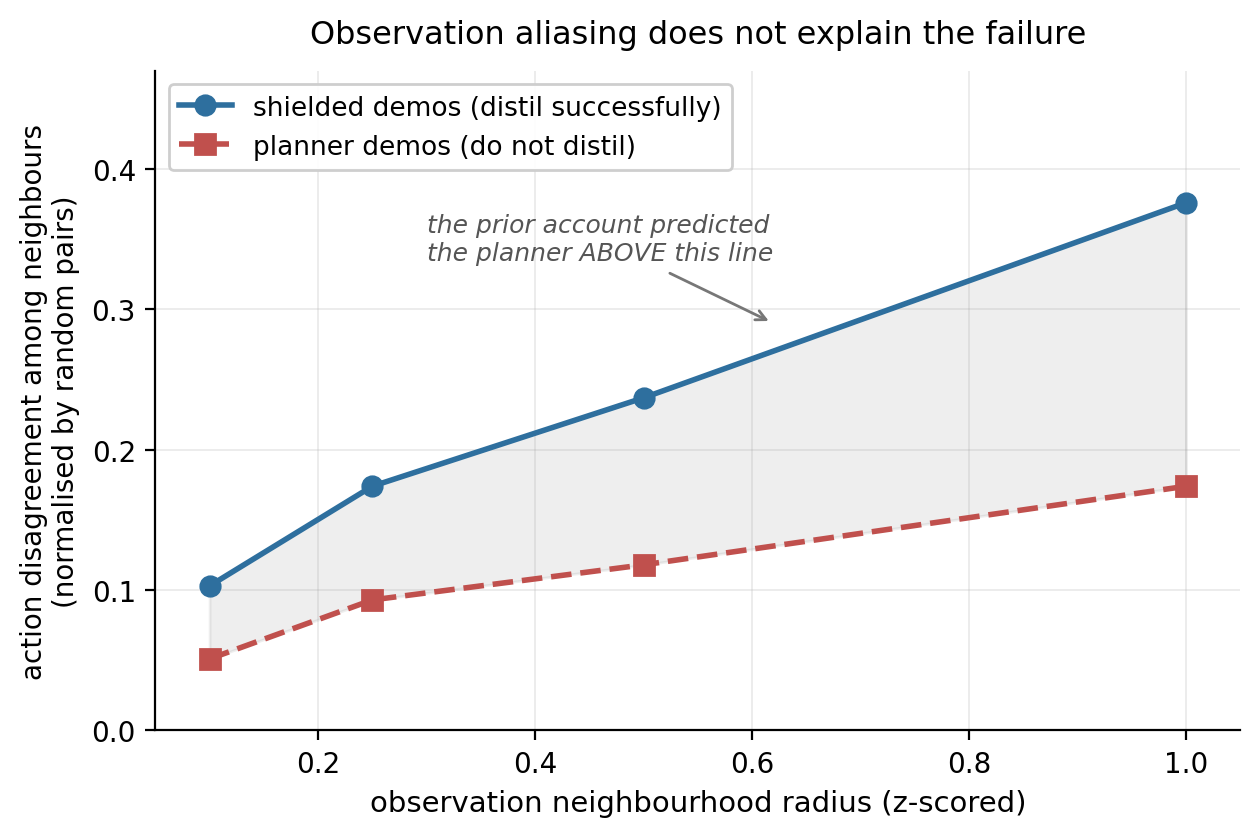
\includegraphics[width=0.72\linewidth]{figures/fig_aliasing.png}
  \caption[Observation aliasing does not explain the transfer failure]{%
    A prediction of this project, refuted by its own data. If the planner's corrections were
    poorly determined by what the policy observes, its curve would lie \emph{above} the shielded
    one. It lies consistently below, by a factor of roughly two at every radius.}
  \label{fig:aliasing}
\end{figure}

\paragraph{Where the teacher had nothing to say.}
Six of the 24 scenes contain no planner demonstrations, so roughly 30 of the 120 evaluation
rollouts test whether the expert could solve the scene at all rather than whether distillation
worked. The gap is systematic rather than random --- the planner fails entirely on
elevated-target tasks, a kinematic limit of the controller rather than a collision-avoidance
one (Appendix~\ref{app:controller}). Restricting to the 18 scenes with training data does not
change the outcome, but both slices are worth distinguishing: the 24-scene figure conflates
scenes where the teacher had nothing to say with scenes where it spoke and was not understood.

\paragraph{Answering RQ3, second part.}
The source of the demonstrations determines whether the transfer occurs. Corrections of equal
density applied to a different controller's trajectories produced no measurable improvement, under
a comparison in which the demonstration source was the only variable. The measured difference
between the two sources is state coverage; observation aliasing was tested as an alternative
explanation and rejected.

\section{What Can the Shield Not Reach?}\label{sec:res:scope}

The shield reduces collisions to 13.3\% but not to zero. This section identifies what the residual
consists of, using per-body collision decomposition. 

\begin{table}[htbp]
\centering
\begin{threeparttable}
\caption[Residual collisions by culprit body]{%
  Per-body attribution of collisions in 120 episodes.}
\label{tab:culprits}
\begin{tabular}{lrrrr}
\toprule
\textbf{Policy} & \textbf{Collided} & \textbf{Gripper} & \textbf{Arm link}
  & \textbf{Held object} \\
\midrule
Base, no shield        & 99 & 71          & 17 & 36 \\
Base + shield          & 16 & \textbf{0}  & 15 & \phantom{0}0 \\
\addlinespace[2pt]
Round 1, no shield     & 23 & \phantom{0}7 & 13 & \phantom{0}9 \\
Round 1 + shield       & 10 & \textbf{0}  & \phantom{0}8 & \phantom{0}1 \\
\addlinespace[2pt]
Round 2, no shield     & 21 & \phantom{0}8 & \phantom{0}8 & \phantom{0}7 \\
Round 2 + shield       & 11 & \textbf{0}  & \phantom{0}9 & \phantom{0}0 \\
\bottomrule
\end{tabular}
\end{threeparttable}
\end{table}

The split is the one Section~\ref{sec:barrier} predicts. Where the barrier's model is precise and
the constrained velocity is the commanded one --- the end-effector --- collisions are eliminated
outright: not one gripper contact across 360 shielded episodes, so the discrete-time
approximation of Section~\ref{sec:shield} holds in practice. Where the model is coarse and the
velocity is inferred, they persist: arm links account for 15 of the 16 residual collisions in the
shielded baseline.

This bears on how Section~\ref{sec:res:internalise} should be read. The distilled policy's
shield-free figure sits within a few points of what its teacher actually achieved, not of a
perfect one --- the teacher's ceiling is set by approximation error in the constraint rather than
by an absence of authority.

\paragraph{The student exceeds its teacher.}
Arm-link collisions fall from 17 to 8 between the base and twice-distilled policies, while the
shielded baseline --- with those same constraints active --- still records 15. The student is
therefore not merely reproducing the filter's corrections: in the channel where the barrier is
least able to enforce anything, it does better than the barrier does.

The likely route is the retention criterion rather than the correction signal. Demonstrations
were kept only if nothing at all was displaced, arm links included, so the dataset encodes
whole-body avoidance that no constraint row ever expressed. Safety reaches the policy through
two channels --- imitation of corrections where the filter has authority, and outcome selection
where it does not --- and only the second can carry behaviour the barrier cannot represent.

This is stated with less confidence than the gripper result: 17/120 against 8/120 is
14.2\% [9.0, 21.5] versus 6.7\% [3.4, 12.6], and those intervals overlap.


\paragraph{Answering RQ4, first part.}
The transfer does not cover the arm links. Where the barrier's model of the robot is precise and
the constrained velocity is the one commanded, collisions are eliminated outright; where the model
is coarse and the velocity inferred, they persist, accounting for 15 of the 16 residual collisions
under the shield. The distilled policy nonetheless improves on its teacher in that channel, on
overlapping intervals.

\section{Are There Other Channels for Safety?}\label{sec:res:channels}

Four further mechanisms were tested.
Table~\ref{tab:negatives} summarises them.

\begin{table}[htbp]
\centering
\begin{threeparttable}
\caption[Mechanisms tested and rejected]{%
  Mechanisms tested and rejected, with the scope at which each negative is claimed. None is a
  general claim about its method class.}
\label{tab:negatives}
\footnotesize
\begin{tabular}{p{0.17\linewidth}p{0.24\linewidth}p{0.22\linewidth}p{0.27\linewidth}}
\toprule
\textbf{Mechanism} & \textbf{What was tested} & \textbf{Outcome} & \textbf{Scope of the negative} \\
\midrule
Scalar-reward RL
  & Flow-SDE GRPO on the action head, 4 configurations $\times$ 6 rounds, one scene
  & Either collapses to inaction or learns nothing; no setting does both
  & The reward design and budget tested. Not safe RL as a class; constrained-MDP and
    world-model methods supply richer signals \\
\addlinespace[3pt]
Language-expressed constraint
  & One safety clause appended to the instruction, $n=60$ per condition, level II
  & No safety change; 23\% slower, 11.7 points less successful
  & The single phrasing tested: generic, unnamed referent, manner adverbial \\
\addlinespace[3pt]
Best-of-$N$ selection
  & $K \in \{4, 8\}$ candidates re-simulated per query, exact state rewind
  & No safe candidate on $\sim$60\% of queries; doubling $K$ buys 8.8 points
  & This policy and benchmark. The measurement it yields is reported as the result \\
\addlinespace[3pt]
Generative uncertainty as a runtime monitor
  & Three statistics of the stored flow-denoising chain, scored as AUC for predicting whether an
    episode collided
  & At chance for the base policy (0.461). The distilled policy inverts consistently
    (0.350, i.e.\ 0.65 flipped) but on 23 collision episodes
  & This policy and benchmark, and episode-level prediction. The inversion is roughly two standard
    errors from chance and is reported as suggestive \\
\bottomrule
\end{tabular}
\begin{tablenotes}[flushleft]\footnotesize
\item A further \emph{explanation}, as opposed to a mechanism, was also tested and rejected:
  observation aliasing does not account for the transfer boundary
  (Section~\ref{sec:res:source}).
\end{tablenotes}
\end{threeparttable}
\end{table}

\subsection*{Scalar-reward reinforcement learning}

RL was tried first, and its failure motivated the imitation approach.

The setup was flow-SDE GRPO on $\pi_{0.5}$'s flow-matching action head: the deterministic sampling
ODE is converted to an equivalent SDE so that log-probabilities exist and a policy gradient can be
taken. A LoRA adapter on the action head received gradients with the backbone frozen, matching the
trainable surface used for distillation in Section~\ref{sec:res:internalise}, so the comparison
between the two learning signals is not confounded by capacity. Rollouts used the CPS sampler at
noise 0.7 with ten denoising steps and clipping 0.2, on one level-II scene, with $K = 8$ rollouts
per group over six rounds. The reward combined success, direct collision, CBF activation rate and
progress terms.

\begin{figure}[htbp]
  \centering
  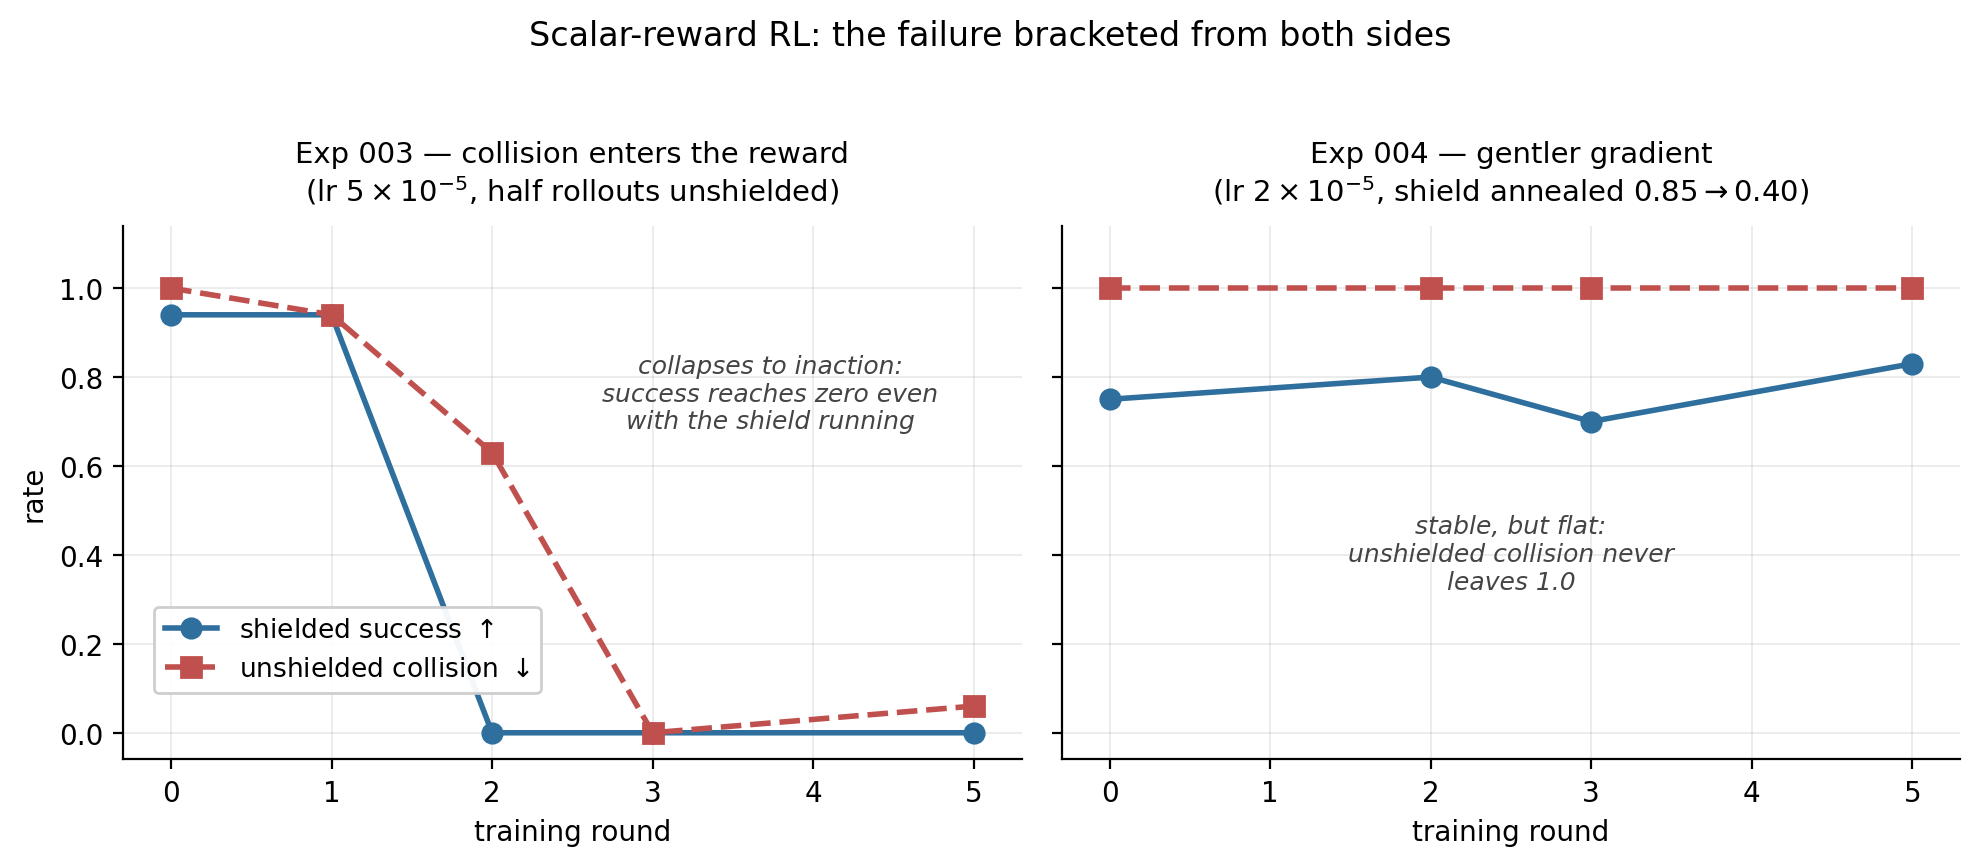
\includegraphics[width=\linewidth]{figures/fig_rl_bracket.png}
  \caption[Scalar-reward RL bracketed from both sides]{%
    The two informative configurations. \textbf{Left:} admitting real collisions to the reward
    moves the policy and it collapses to inaction --- success reaches zero even in the shielded
    condition, which the shield alone cannot cause. \textbf{Right:} a lower learning rate with an
    annealed shield fixes the collapse and learns nothing.}
  \label{fig:rl_bracket}
\end{figure}

Two configurations bracket the failure. With the shield active on every rollout, collisions never
enter the reward directly --- the shield prevents them --- so the only safety signal is the
activation penalty, and raising the learning rate to $5 \times 10^{-5}$ with the activation weight
at 1.5 left the policy flat. Running half of each group's rollouts unshielded admits real
collisions and widens the within-group spread to roughly $\Delta = 1.0$; the safety metric improved
immediately and the task collapsed with it, as the adapter diverged under a far higher-variance
reward and the collision penalty suppressed forward motion, which in these scenes almost always
collides early in training.

These are not two settings with a working point between them. The only configuration that moved the
policy's behaviour collapsed it, and every configuration stable enough to preserve the task learned
no avoidance, because the learning signal and the destabilising signal are the same knob. A scalar
episode reward gives no per-step spatial credit, so the policy cannot separate detouring around the
obstacle from stopping short of the goal when the obstacle lies on the path to it; and in a
flow-matching policy exploration \emph{is} sampling noise, which is also what degrades the actions
being evaluated. This is what the shield supplies and the reward cannot: the barrier computes the
correct action at every step it intervenes, in the space the policy emits, so credit assignment is
given rather than inferred.

\subsection*{Safety expressed in language}

The experiment has the same checkpoint, seed, held-out initial states and
evaluation code for both conditions, differing only in a safety clause appended to the instruction. Twelve
level-II scenes at five initial states each give $n = 60$ per condition; level II was chosen
because of difficulty calibration.

\begin{quote}\small
\textbf{plain:} \texttt{pick up the black bowl between the plate and the ramekin and place it on
the plate}\\[3pt]
\textbf{safety:} \texttt{\dots{} and place it on the plate, being careful not to touch or knock
over any other objects}
\end{quote}

The phrasing is generic: it names no object, gives no spatial reference, and
states the constraint as a manner adverbial rather than a prohibition.

\begin{table}[htbp]
\centering
\caption{Effect of appending a safety clause to the instruction. $n = 60$ per condition, twelve
  level-II scenes, Wilson 95\% intervals.}
\label{tab:language}
\begin{tabular}{lccc}
\toprule
\textbf{Condition} & \textbf{TSR (95\% CI)} & \textbf{Collision (95\% CI)} & \textbf{ETS} \\
\midrule
Plain instruction       & 66.7\% [54.1, 77.3] & 70.0\% [57.5, 80.1] & 132.4 \\
Safety clause appended  & 55.0\% [42.5, 66.9] & 68.3\% [55.8, 78.7] & 162.4 \\
\bottomrule
\end{tabular}
\end{table}

The policy responds to the safety clause by marginally  decreasing collisions, succeeding less often, and taking longer to complete. 

The natural reading is that safety language elicits a general behavioural prior --- hesitancy,
reduced speed --- rather than a grounded avoidance behaviour. The model has learned that
safety-flavoured instructions correspond to cautious-looking motion, and that association is not
connected to the geometry of the scene.

ROAD-VLA got similar negative results from their text-based grounding experiments~\cite{wang2026roadvla}. They attribute the failure to a modality gap preventing discrete text from supplying the grounding continuous control requires.

\subsection*{Best-of-$N$ selection}

If safety varied across the actions a policy might sample from a given state, it could be obtained
by rejection: draw $K$ candidate action chunks, simulate each, execute the safest. The sampler must
be stochastic for candidates to differ, so the matched control is $K = 1$ at the same noise level
rather than the deterministic policy used elsewhere in this chapter. Making the measurement
trustworthy required the simulator to be rewound exactly between candidates; snapshot and restore
were verified to machine precision before any result was recorded.

\begin{figure}[htbp]
  \centering
  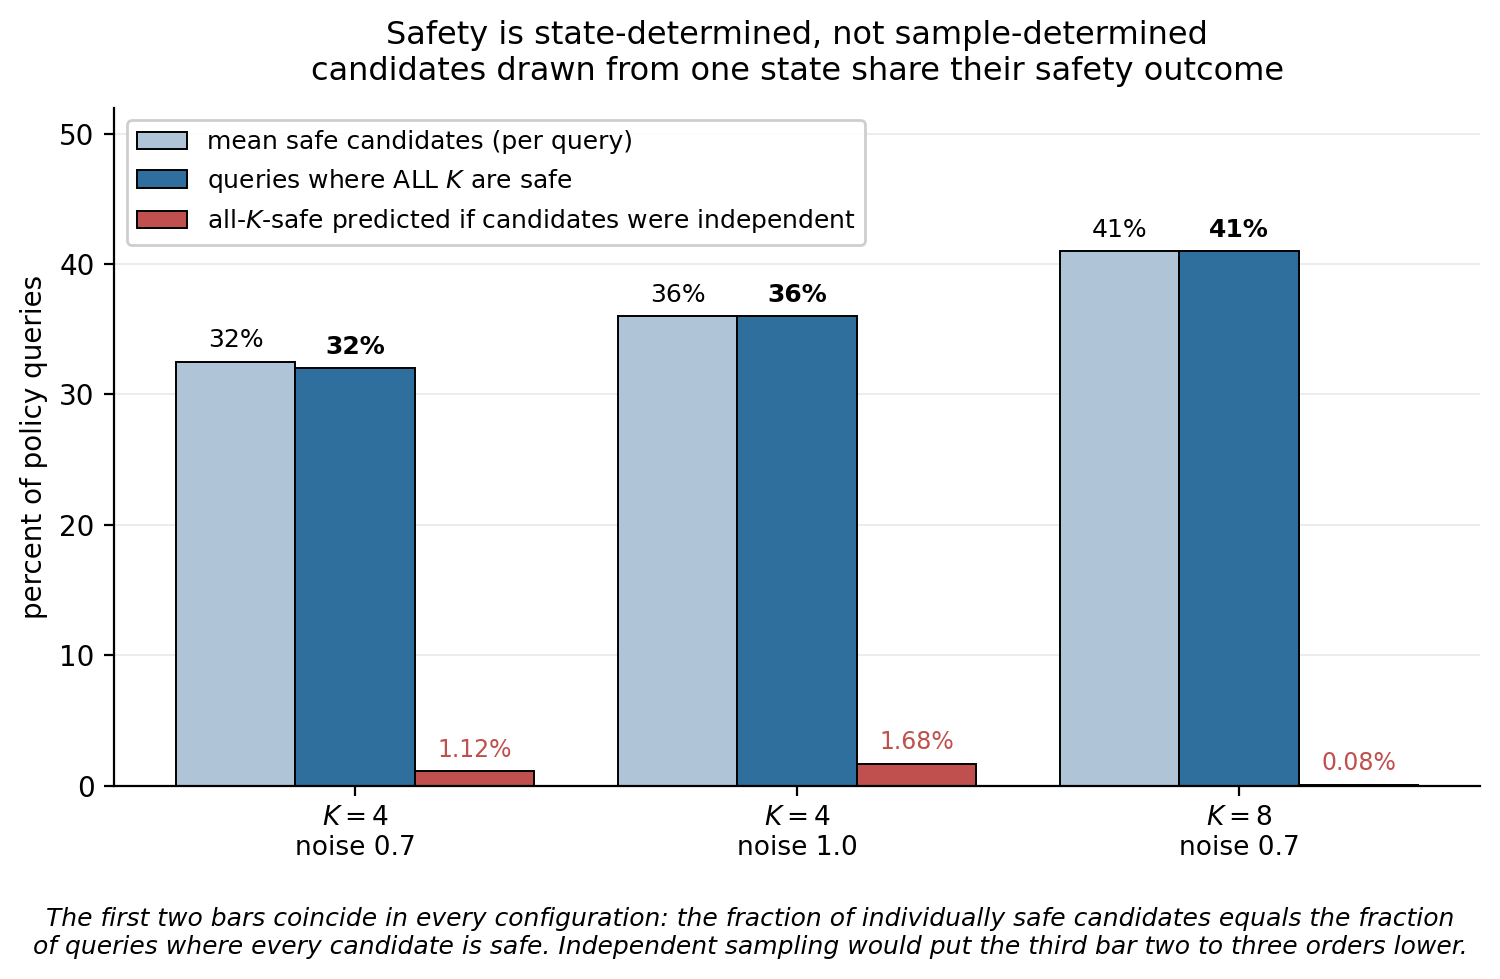
\includegraphics[width=0.82\linewidth]{figures/fig_bon_correlation.png}
  \caption[Within-state safety correlation in a VLA policy]{%
    Why rejection sampling cannot help here. In every configuration the fraction of individually
    safe candidates coincides with the fraction of queries in which \emph{all} $K$ are safe, so a
    query is $0$-of-$K$ or all-of-$K$ safe and almost never in between. Independent sampling would
    make the all-$K$-safe rate two to three orders of magnitude smaller (right-hand bars).}
  \label{fig:bon}
\end{figure}

As a method this is negative: on roughly 60\% of queries no candidate was safe, and buying more
candidates barely moved it --- doubling $K$ from four to eight recovered 8.8 percentage points for
twice the compute, and raising the noise recovered 3.7.

The measurement underneath it is the more interesting result. The mean safe fraction and the
all-$K$-safe fraction coincide in all three configurations. Were the candidates independent draws,
the all-$K$-safe rate would be $p^{K}$: 1.1\% at $K = 4$ and 0.08\% at $K = 8$, against observed
values of 32\% and 41\%. The policy's samples from a given state are therefore near-perfectly
correlated in their safety outcome.

Safety in this policy is consequently \textbf{state-determined rather than sample-determined}, at
least on this benchmark. Once a state is reached the outcome is largely fixed, and no amount of
choosing among actions recovers it --- the leverage lies in not reaching the state. This also
explains a result that would otherwise look inconsistent: episode-level filtering worked
(Section~\ref{sec:res:mechanism}) while action-level selection cannot, because episode-level
selection chooses between trajectories that reached \emph{different states}, which is the axis
along which variation actually exists.

The correlation measurement is offered here as the contribution rather than the selection method.
It is, as far as this work is aware, the first measurement of candidate-level safety correlation in
a VLA policy, and it is the sharpest available statement of the reachability
theme running through Sections~\ref{sec:res:scope}, \ref{sec:res:mechanism} and the discussion that
follows.

\subsection*{Generative uncertainty as a collision predictor.} Uncertainty was also tested as a barrier-free monitor: $\pi_{0.5}$ stores the full denoising chain
for every action, and if the policy were less certain where safe and unsafe behaviours are both
plausible, that chain would carry a risk signal requiring no obstacle geometry at all. It does
not --- the association is at chance for the base policy, and the distilled policy's consistent
\emph{inversion} suggests, on limited evidence, that its remaining failures are confident ones.

\paragraph{Answering RQ4, second part.}
None of the four alternatives substituted for shielded imitation under the implementations and
budgets tested. Each negative is scoped as stated in Table~\ref{tab:negatives}, and one of them
yields a measurement rather than a method: within a given state, the safety outcomes of the
policy's sampled action candidates are near-perfectly correlated.

\section{Conclusion}\label{sec:res:conclusion}

This chapter reported the experiments in the order of the research questions. A control barrier
function shield makes $\pi_{0.5}$ substantially safer on this benchmark, and reproduces the
published baseline closely enough to validate the evaluation pipeline (RQ1). Distilling the
shielded policy's own corrected rollouts internalises that safety: with no shield at inference the
policy is both safer and more successful than the model it came from, recovering most of the
shielded baseline's collision avoidance in a single round (RQ2).

Two controls bound that result. The improvement is attributable to the shield's corrections rather
than to outcome selection, and it does not survive a change of demonstration source: a
geometry-privileged planner supplying corrections of equal density produced no measurable gain
(RQ3). The transfer leaves the arm links largely uncovered, and four alternative mechanisms --- 
scalar-reward reinforcement learning, language-expressed constraints, best-of-$N$ selection and
uncertainty monitoring --- failed to substitute for it (RQ4).

Chapter~\ref{ch:discussion} interprets these findings, sets them against the literature of
Chapter~\ref{ch:background}, and states what they do and do not establish.
